\documentclass[12pt]{HomusWorkus}

\begin{document}

% ------------------------------------------------------------
%           Титульна сторінка
% ------------------------------------------------------------
\begin{titlepage}
    % \begin{figure}
    %     \centering
    %     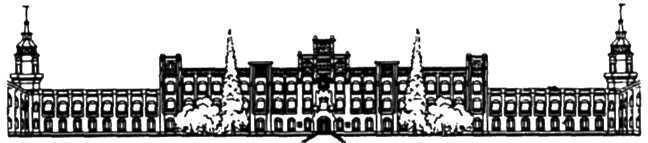
\includegraphics[scale=0.6]{Images/kpi_1.png}
    % \end{figure}

    \begin{center}
        \small{\textbf{НАЦІОНАЛЬНИЙ ТЕХНІЧНИЙ УНІВЕРСИТЕТ УКРАЇНИ\\
        «КИЇВСЬКИЙ ПОЛІТЕХНІЧНИЙ ІНСТИТУТ імені ІГОРЯ СІКОРСЬКОГО»\\
        НАВЧАЛЬНО-НАУКОВИЙ ФІЗИКО-ТЕХНІЧНИЙ ІНСТИТУТ\\
        }}
        
        \vfill
        \Huge{\textbf{СУЧАСНI АЛГЕБРАЇЧНI КРИПТОСИСТЕМИ}}

        \vspace{0.2cm}
        \large{\textbf{КОМП’ЮТЕРНИЙ ПРАКТИКУМ}}

        \vspace{0.2cm}
        \large{\textit{
            Дослiдження сучасних алгебраїчних криптосистем
        }}
        
        % \vspace{0.2cm}
        % \large{\textbf{Варіант 1}}

        \vfill
        \large{
            \begin{flushright}
                \begin{tabular}{l}
                    \hskip-0.5cm \textbf{Виконали:}  \\
                    Волинець Сергій ФІ-42мн \\
                    Сковрон Роман ФІ-42мн \\
                    % \hskip-0.5cm \textbf{Перевірив:}  \\
                    % Волинець Сергій ФІ-03  \\
                \end{tabular}
            \end{flushright}
        }

        \vfill
        \large{Київ --- \the\year{}}
    \end{center}
\end{titlepage}
\addtocounter{page}{1}

% ------------------------------------------------------------
%           Зміст
% ------------------------------------------------------------
\tableofcontents
\newpage

% ------------------------------------------------------------
%           Основний текст
% ------------------------------------------------------------

\section{Мета}

Дослiдження особливостей реалiзацiї сучасних алгебраїчних криптосистем на прикладi
учасникiв першого раунду процесу стандартизацiї постквантової криптографiї (NIST PQC).

\section{Постановка задачі}

Розробити програмну реалiзацiю алгоритму цифрового підпису ``CRYSTALS-Dilithium''.
Знайти схожi алгоритми та провести порiвняльний аналiз швидкодiї за рiзних умов та використання модифiкацiй складових частин.
Навести повний теоретичний опис алгоритму з усiма деталями та вiдомими результатами дослiджень.
Провести теоретичний порiвняльний аналiз обраного алгоритму зi схожими алгоритмами та дослiдити можливiсть перенесення вiдомих атак на обраний алгоритм.

\section{хiд виконання роботи та опис труднощiв}

\section{Опис криптографiчного алгоритму та його складових частин}

Вступ CRYSTALS-Dilithium — це схема цифрового підпису, заснована на складності задачі пошуку коротких векторів у решітці. Безпека цієї схеми ґрунтується на цій складності. Алгоритм спроектований для забезпечення високого рівня захисту від різних атак, включаючи атаки з використанням квантових комп'ютерів. У порівнянні з іншими схемами на решітках, які потребують складної генерації випадкових чисел за допомогою дискретного гауссівського розподілу, Dilithium спрощує свою реалізацію, використовуючи рівномірний розподіл, що мінімізує ризики вразливостей до атак через побічні канали. Крім того, це збільшує простоту реалізації, а тому він має менші ризики зменшення рівня безпеки, через необережну імплементацію. Алгоритм оптимізований для зменшення розміру публічного ключа та підпису, зберігаючи при цьому модульність для варіативних рівнів безпеки. За словами авторів, він має найменшу сумарну довжину ключа та підпису з існуючих схем підпису на решітках з таким же рівнем безпеки.

\section{Результати порiвняльного аналiзу швидкодiї обраного алгоритму зi схожими алгоритмами}

\section{Огляд наявних результатiв дослiджень обраного алгоритму}

\section{Результати порiвняльного аналiзу стiйкостi обраного алгоритму зi схожими алгоритмами}

\section{Опис тестiв, якi проводилися з метою перевiрки коректностi реалiзованої програми}

\section{Детальний опис особливостей реалiзацiї та приклади застосування}

\section{Результати аналiзу постквантової стiйкостi за наявними результатами аналiзу}


\section{Висновки до роботи}



% ------------------------------------------------------------
%           Bibliography
% ------------------------------------------------------------
% \bibliographystyle{alpha}
% \bibliography{sample}

\end{document}
